\section{Results}
We developed a few different Parkour movements to demonstrate the
generality of our framework. All the results shown in the video were
produced on a single core of 3.20GHz CPU. Our program runs at $1000$
frames per second with the time step of $0.5$ millisecond. We used
RTQL8 \cite{RTQL8:2012:URL}, an open-source simulator for multibody
dynamics based on generalized coordinates. The character has $33$
degrees of freedom. Except for the first six degrees of freedom that
describe the global translation and orientation, all other degrees of
freedom can be actuated.  

\begin{table}[ht]
  \center
  \caption{Instructions used to train a precision jump.}
  \begin{tabular}{ | p{3.0cm} | p{7.0cm} | }
    \hline
    Phase & Instruction \\ \hline
    Leaning & MOVE downward BY $0.1$m \\ \hline
    Leaning & MOVE downward BY $0.2$m \\ \hline
    Leaning & head IN FRONT OF root \\ \hline
    Thrusting & SPEED near $[1.2, 2.4, 0.0]^T$ \\ \hline
    Thrusting & SLOWDOWN 20\% \\ \hline
    Thrusting & spin about z FORWARD \\ \hline
    Airborne &  PLACE feet NEAR $[0.8, 0.0, 0.0]^T$ \\ \hline
    Airborne & PLACE COM NEAR $[0.7, 0.4, 0.0]^T$ \\ \hline
    Airborne & MOVE upward BY $0.1$m \\ \hline
    Landing & PLACE COM NEAR $[0.7, 0.5, 0.0]^T$ \\ \hline
    Landing & BALANCE \\ \hline
    All & RELAX arms BY 30\%\\ \hline
    Leaning & FLEX elbows BY $20^\circ$ \\ \hline
    Airborne & FLEX elbows BY $80^\circ$ \\ \hline
  \end{tabular}

  %% \caption{Instructions for training a precision jump}
  \label{tab:parkour_instructions}
\end{table}

\subsection{User Input}
Our system requires the user to break down a complex motion into
phases and provide an initial controller for each phase. Determining
the phases of a motion is at the user's discretion. In our
experiments, we simply used the timing of contact change to determine
phases. Similarly, the initial controllers do not have significant impact
on the final controllers. All the initial
controllers we used in our experiments were simple PD controllers with
the same gains and damping coefficients. The
only goal of each controller was to track a single target pose roughly defined
by the user (\figref{parkour_keyframes}).

%% \updated{ Also, our system is not sensitive to the selection of
%%   instructions.  For instance, in the scenario of training a precision
%%   jump (Table \ref{tab:instructions}), the user could overwrite the
%%   previous instructions (The third instruction replaces the second),
%%   or use the different instruction which has same effect (The fourth
%%   instruction can be replaced by ``Torso orientation about z GREATER
%%   THAN 0'').  However, still resolving subtle issues for complex
%%   motions can be difficult for a non-expert.  This is also true for
%%   learning motions in real world: a better coach can diagnose problems
%%   in your movement more precisely and effectively.  } 

During the training process, the user needs to provide instructions
iteratively to improve the motor skill of the character. However, we
observed that the character could successfully learn a motor skill,
even when the instructions were clearly not optimal. For example, in
the scenario of training a precision jump (Table \ref{tab:parkour_instructions}),
the user gave repetitive commands using ``MOVE downward BY'' instruction
to adjust the leaning angle of the character.
For more complex cases, we believe that the user's
prior knowledge about the motion will become an important factor. This
is also true for learning motions in real world; a better coach can
diagnose problems of the movement more precisely and effectively.  

When the user gives conflicting instructions,
such as ``SPEEDUP 200\%'' and ``TRANSLATE torso backward'',
the optimizer will yield a solution which tries to achieve both conflicting goals,
but the resulting motion could be undesirable or unpredictable.


\subsection{Training Dynamic Skills}

\begin{figure}[tb]
\center
  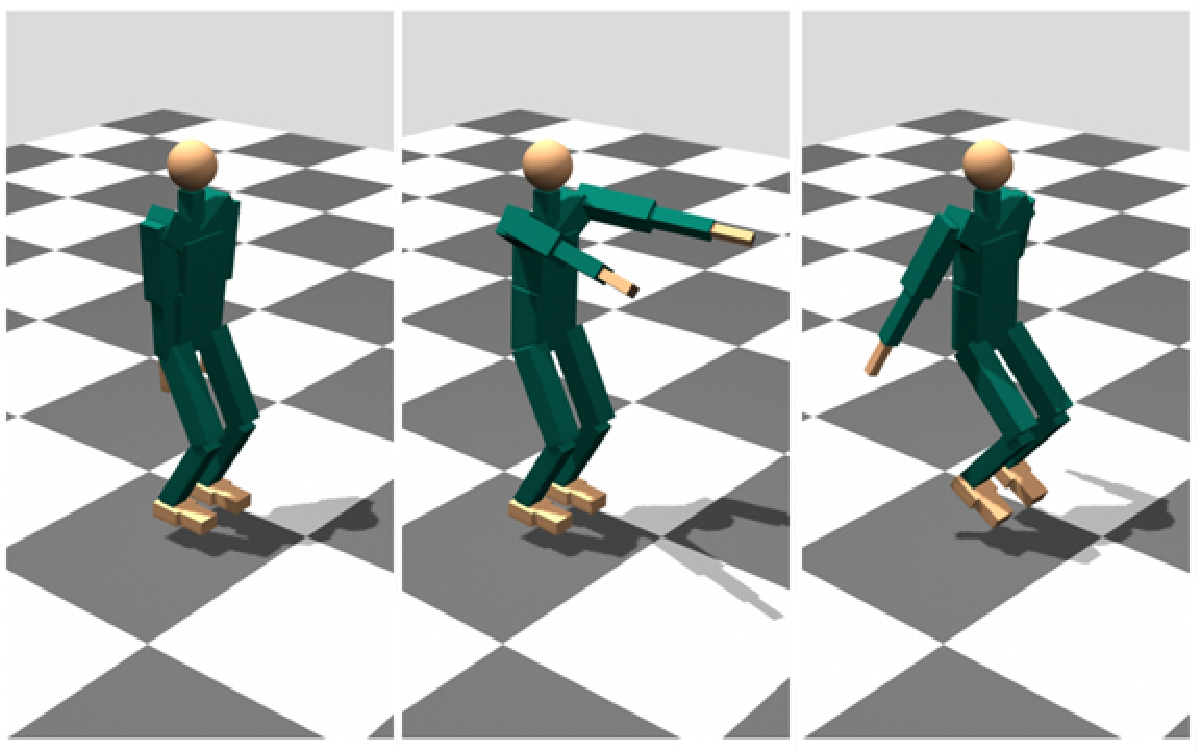
\includegraphics[width=4.2in]{images/keyframes}
  \caption{
    We use these three target poses for all the initial
    controllers, except for the rolling phase of drop-and-roll.
  }
  \label{fig:parkour_keyframes}
\end{figure}

\myparagraph{Precision Jump}
A precision jump is a jumping motion that lands on a narrow target,
such as the top of a wall or a rail. The precise distance and the
smaller target require more accurate and coordinated control. We broke
the entire sequence into four phases based on the contact state:
leaning, thrusting, airborne, and landing. We trained each phase
separately and applied parameterization and concatenation technique
to sequence them into one controller for precision jump.
The final state of the motion satisfies the balance condition,
which limits the ground projection of center of mass within the suppor
polygon and the velocity of center of mass to near zero.


The initial controller for each phase was a simple PD controller
tracking a roughly designed pose (Figure \ref{fig:parkour_keyframes}). Because
of the lack of control on the global state, the initial controller
resulted in falling motion immediately. In all of our examples, we
designed initial controllers in the same fashion.

Training all four phases took $14$ instructions in total. We listed all
the instructions in Table \ref{tab:parkour_instructions}. For each phase, the average
number of control rigs used was $3.25$, which resulted in $4.25$ rig
parameters to optimize. The optimization time for each phase on
average took two minutes. The task parameters we used for parameterizing
four phases are the leaning angle, thrusting direction, and airborne
traveling distance. The average time spent on parameterization of one
phase is 30 minutes.

During the coaching stages, we first gave instructions to guide global
motion so the character can successfully perform the jump
without falling. Later, we added instructions to modify styles on the
upper body. The instructions we used might not be the most effective
ones because we are not experts in Parkour. For example, we used a few
consecutive instructions to lower the center of mass, which could have
been done in one instruction. Similarly, we instructed the character
to flex the elbows in the leaning phase and later added the same style in
the airborne phase. Although the total number of instructions can be
reduced, our goal here is to demonstrate how this framework is used by
a non-expert who tends to give imprecise and incremental instructions
based on the feedback from the trainee.


\myparagraph{Turnaround Jump}
A turnaround jump requires the performer to jump in place while
turning in a precise angle. Although it consists of the same four phases
as a precision jump, the difference is that it involves asymmetric
motion and the control of angular momentum.

In our experiment, training all phases of a turnaround jump required
nine instructions. For each phase, the average number of control rigs
was $3.75$ and the average number of rig parameters was $4.75$. The
optimization time for each phase was on average one minute. We
parameterized the thrusting angular momentum, which took 12 minutes to
complete.

We found that the coaching skill of the human user can also improve by
using this framework. Because of our previous experience in coaching a
precision jump, we used fewer instructions to train a turnaround
jump. We also gained better insight on developing more natural landing
controller. That is, we instructed the character to raise its center
of mass at landing so that the character had more room to absorb the
impact.

\begin{figure*}[htbp]
\center
  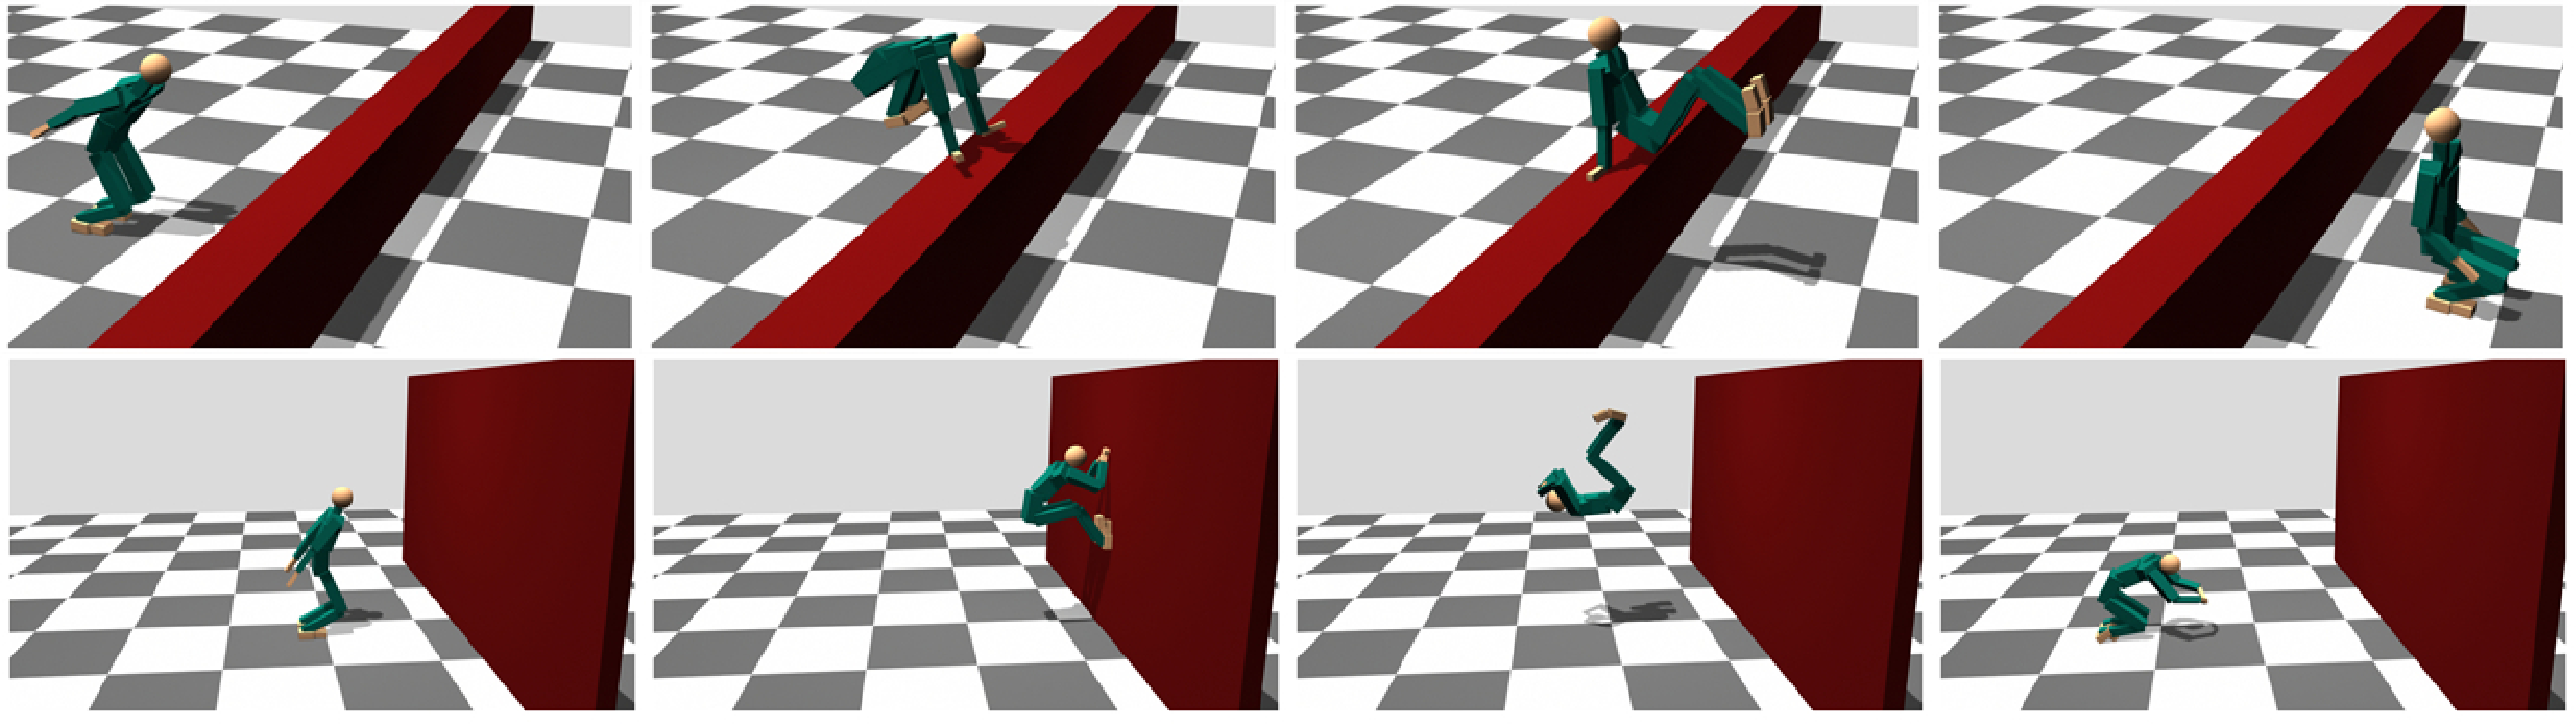
\includegraphics[width=0.95\linewidth]{images/results}
  %% 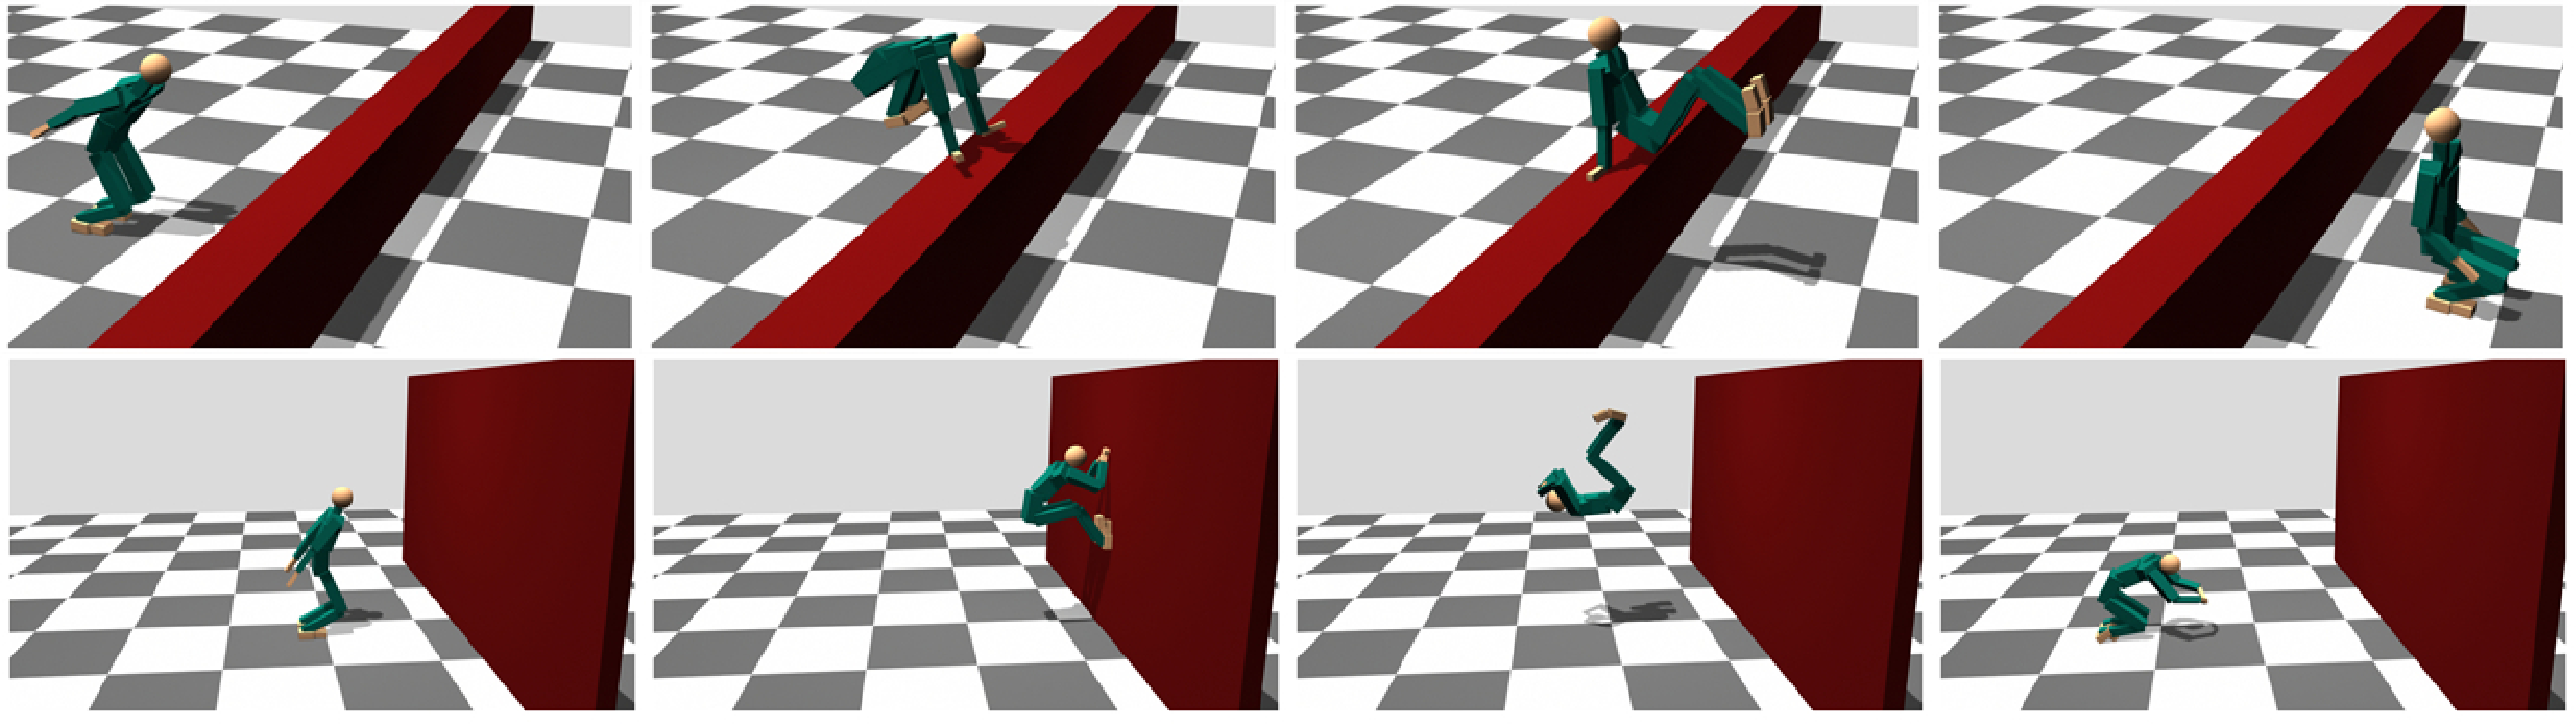
\includegraphics[width=6.7in]{images/results}
  \caption{
    Monkey vault and wall-backflip.
  }
  \label{fig:parkour_results}
\end{figure*}

\myparagraph{Monkey Vault}
A monkey vault is a basic Parkour movement for getting over obstacle
without slowing down the motion (Figure \ref{fig:parkour_results}).
The performer approches the obstacle
with squat position and uses the hands to reach for the vault. As the
performer jumps in the air, s/he leans forward and tucks the legs
against the upper body. Since the hands are placed wider than the
shoulder width, the legs can pass through in between the arms. We
broke the vaulting motion into six phases: leaning, thrusting,
airborne, pushing, extending, and landing.

Training all six phases of a monkey vault took $26$ instructions.  For
each phase, the average number of control rigs was $2.33$ and the
average number of rig parameters was $3.66$.  The optimization time
for each phase was on average three minutes. We parameterized the monkey
vault controller by its leaning angle, thrusting direction, pushing
direction, and extending velocity. The computation time for
parameterization was 40 minutes for each phase.

Training a monkey vault was the most challenging task among all our
experiments because our intuition of monkey vault was
limited. For example, it was not clear to us when the character should
accelerate or which direction the character should push. The
instructions we used were more back-and-forth and repetitive due to
our unfamiliarity to this motor skill.

\myparagraph{Drop-and-roll}
The purpose of rolling in Parkour is to protect joints from
the landing impact. We designed a rolling controller from a standing
position and later showed that it can be concatenated to a precision
jump or a monkey vault to complete a drop-and-roll motion. We broke
the rolling motion to three phases: leaning, thrusting, and follow-through.

Training the entire rolling motion required eight instructions.  For each
phase, the average number of control rigs was $2.66$ and the average
number of rig parameters was $4.66$. The optimization time for each
phase was on average 1 minute. We parameterized the rolling controller
by the leaning angle and the angular momentum at the thrusting
phase. The computation time for parameterization was about ten
minutes for each phase.

Developing a drop-and-roll controller is relatively easy because it has
only three phases and the follow-through phase is very passive. As
long as the angular momentum is sufficient, the character naturally
goes into rolling motion.
 
\myparagraph{Wall-backflip}
A wall-backflip is a combination of a wall-run and a backflip
(Figure \ref{fig:parkour_results}). The performer jumps toward the wall, kicks
the wall at contact, flips backward in the air, and lands on both
feet. We broke the task into six phases: leaning, thrusting, airborne,
kicking, flipping, and landing.

Training all six phases require $18$ instructions.  For each phase,
the average number of control rigs was $2.66$ and the average number
of rig parameters was $4.00$.  The optimization time for each phase
was on average two minutes. We parameterized the controller by the
angular momentum at the kicking phase. The computation time for
parameterization was about 30 minutes for each phase.

The experience of coaching monkey vault greatly helped us to train a
wall-backflip. They share similar phases, but the main difference is
that the character needs to maximize the backward angular momentum at
the kicking phase. Without optimization, the direction of the kicking
force would have been a difficult parameter to tune because it must
generate sufficient angular momentum without causing slipping contact.


\subsection{Limitations}
Our controllers are able to withstand some perturbations. For example,
the same precision jump controller trained for landing on the floor
can be applied to landing on a rail. However, most controllers become
unstable when additional push forces are applied to the character. We
suspect that the instability is due to the feedforward nature of
the virtual force control rig.

Using contact states to break a task into smaller phases is a good
strategy for the examples we demonstrated, but it is not sufficient
for more complex and timing-sensitive motor skills, such as tic-tac or
wall-run. These movements switch controllers not only based on
contact states, but also on character's pose, speed, or spatial
relation to the environment. One possible solution is to design more
sophisticated control rigs which include time-varying rig parameters.

In the absence of a running controller, we were not able to generate
some motor skills which require a high initial forward momentum to
carry out the motion smoothly. We believe that the monkey vault motion
can be largely improved if we concatenate it with an adequate running
controller.

Although the performance of CMA-C on our Parkour problems is
five times faster than the standard CMA on average, the large
variance in performance gain (150\% to 650\%) indicates that further
evaluation on a broader set of benchmark problems is needed. Our toy
problems do not provide comprehensive analyses on CMA-C because they
made specific assumptions about the shape of the cost functions,
such as asymmetric random noise or symmetric undulation. These
assumptions may not reflect the true landscape of the cost functions
in the Parkour problems. We conjecture that the success of CMA-C on the
Parkour problems is due to the large infeasible regions and multiple
local minima in the cost functions, which may cause standard CMA to
converge slower.

  %% We also analyzed the few selected Parkour problems, and our experience indicates
  %% that 
  %% However, their landscapes of enery functions are not yet fully explored
  %% due to their high dimensionality, so more detailed analysis is required
  %% to prove the robustness of CMA-C.}





